\documentclass{article} %this is an article
\usepackage[lmargin=.75in,rmargin=.75in,tmargin=1.in,bmargin=1in]{geometry} % setting margins
%\usepackage{tree-dvips}
\usepackage{tikz}  %makes crazy graphs
\usepackage{enumitem}
% \usetikzlibrary{snakes}
%\usepackage[flushleft]{threeparttable} %% makes notes for tables that wraps around width of table
%\usepackage{chronology}
\usepackage[round]{natbib}  %% beatiful bibliography
%\usepackage{wrapfig}
%\usepackage{longtable} %%multipage table
%\usepackage{qtree}
\usepackage{verbatim} %all kinds of shit
\usepackage{graphicx} %beautiful figures
%\usepackage{graphics}
%\usepackage{color}
%\usepackage{caption}
\usepackage{subcaption} %subcaption on the the subfigures
%\usepackage{multirow}
%\usepackage{sidecap}
%\usepackage{epstopdf}
\usepackage{amssymb} %beautiful math
\usepackage{amsmath,amssymb,amsfonts,amsthm,array} %beautiful math
\usepackage{amsthm}  %beautiful math
\usepackage{pgfplots}  %Normal distribution figure
\usepackage[colorlinks=true,linkcolor=red, citecolor=red]{hyperref} %sets my preferences for cross reference



\begin{document}
\begin{center}
  \textbf{Joao Rodrigues} \\
  \textbf{Economics 8185 - Computational Methods} \\
  \textbf{Homework 3a - Aiyagari (1994)} \\
  \textbf{Economics Department}
\end{center}
\section*{Model details}
In the Aiyagari (1994) economy, there is a continuum of agents who consume $c_t$, save in $a_{t+1}$, value leisure $l_t$ and supply his/her non-leisure time to labor ($1-l_{t}$). The individual problem can be defined for an individual who takes the interest rate $r$ and wage rate $w$ as given according to:
\begin{align*}
  \max_{\{a'_t, l_t\}} & \quad  E\sum_{t=0}^{\infty} \beta^t u(c_t,l_t)    \\
  st:     & \quad c_t + a_{t+1} = (1+r)a_{t} + (1.0-l)w\epsilon   \\
           & \quad a_{t+1} \geq 0
\end{align*}
There is a representative firm who demands labor and capital while also taking prices as given. The firm's technology if Cobb-Douglas and it maximizes profit.Accordingly, we prices must satisfy: 
%%%
$$r = \alpha (L/K)^{1-\alpha} - \delta \Rightarrow w = (1-\alpha)(L/K)^{\alpha} $$
%%%
We'll construct a Stationary rational expectations equilibrium where aggregate savings and labor supply from consumers are used in production by the representative firm. There are prices $r,w$ that rationalize these allocations. Since this is a stationary equilibrium, the distribution of assets is such that this distribution does not change from today to tomorrow.
\section*{Computation}
I start the algorithm with a guess for the equilibrium interest rate and labor
\begin{enumerate}
\item solve the individual problem
\item compute the stationary distribution of assets based on individual decision rules
\item compute capital and labor supply by aggregating individual decisions over the stationary distribution
\item if supply equal demand (implied by aggregate production function), stop, otherwise, update $r$ and $w$ and go back to beginning.
\end{enumerate}
%%%%
In order to solve for the individual policies, I followed closely the methods delineated in Aiyagari \& McGrattan (1998). That is, I used a finite element method with Galerkin weights and linear basis functions to solve for a savings policy. Further, I solved for equilibrium the same way they did, i.e. with a bisection over the interest rate and a newton over the labor supply in an outer loop. Finally, I used Young (2010) in order to compute the transition matrix, and consequently the stationary distribution which, becomes a simple eigenvalue problem on the transition matrix. This means that the stationary distribution is the eigenvector associated with the unit eigenvalue of the transition matrix.\\
\\
I did not do as Aiyagari (1994) who discretized an AR1 process for the idiosyncratic labor income shock. Instead I solved the model as in Marcet et al (2006) with high and low shocks where high shocks had high probability of remaining high while low shocks still had a higher probability of going high but lower than if you came from the high state. Below I solved various versions of the model which illustrates some but not all mechanisms in play. I used the following utility function:
$$u(c,l) = \frac{c^{1-\gamma_c}}{1-\gamma_c} + A\frac{l^{1-\gamma_l}}{1-\gamma_l}$$
technology parameters were kept fixed for all cases solved. I.e. $\alpha = 0.36$ and $\delta = 0.025$
\section*{Results}
\subsection*{Exogenous labor}
For the exogenous case, I'm plotting the distribution and a demonstration of demand and supply moving towards equilibrium.
\begin{figure}[h!]
  \centering
  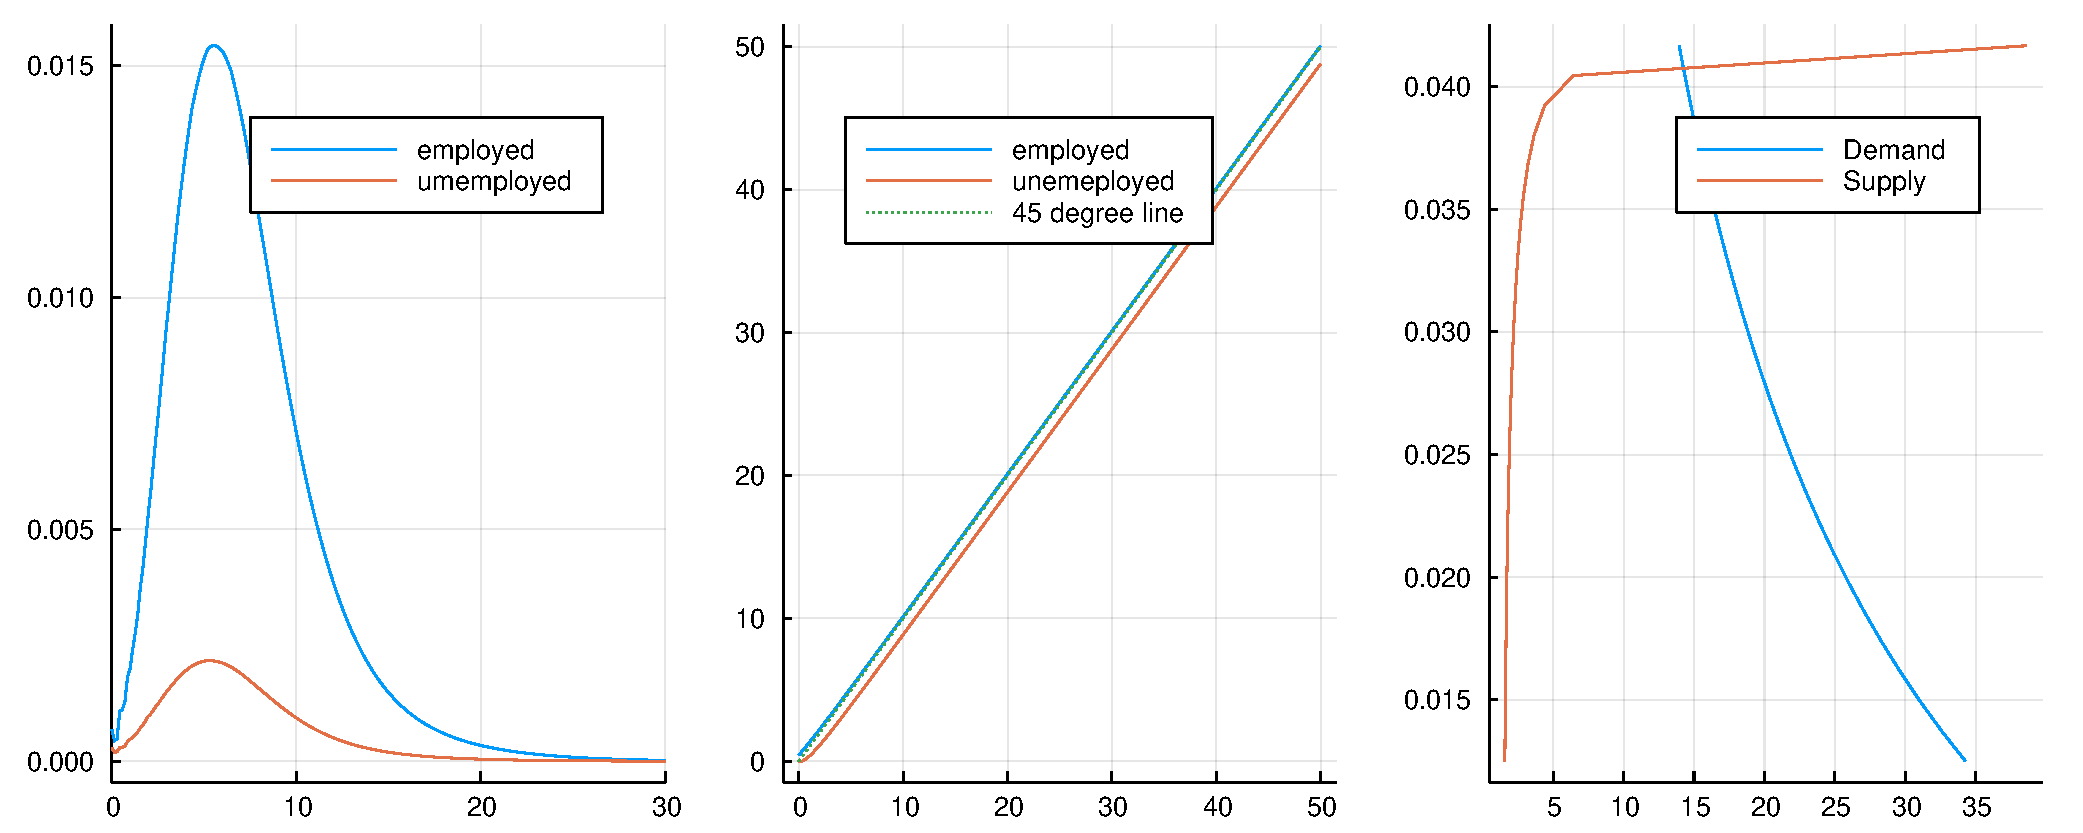
\includegraphics[width = 0.8\textwidth]{../Inelastic/exosolution.pdf}
    \caption{$u(c)=\log(c)$ and $\beta = 0.96$}
  \end{figure}
  The individual policies show that since the agent does not value leisure, he/she can't sacrifice leisure for income, which results in the near parallel policy function for both high and low income shocks. The kink near the origin for the low income agent shows that at very low income, the agent can't save and is borrowing constrained. The mass of the distribution at the origin represent the mass of agents that are borrowing constrained. 
  \subsection*{Valued leisure}
\begin{figure}[h!]
  \centering
  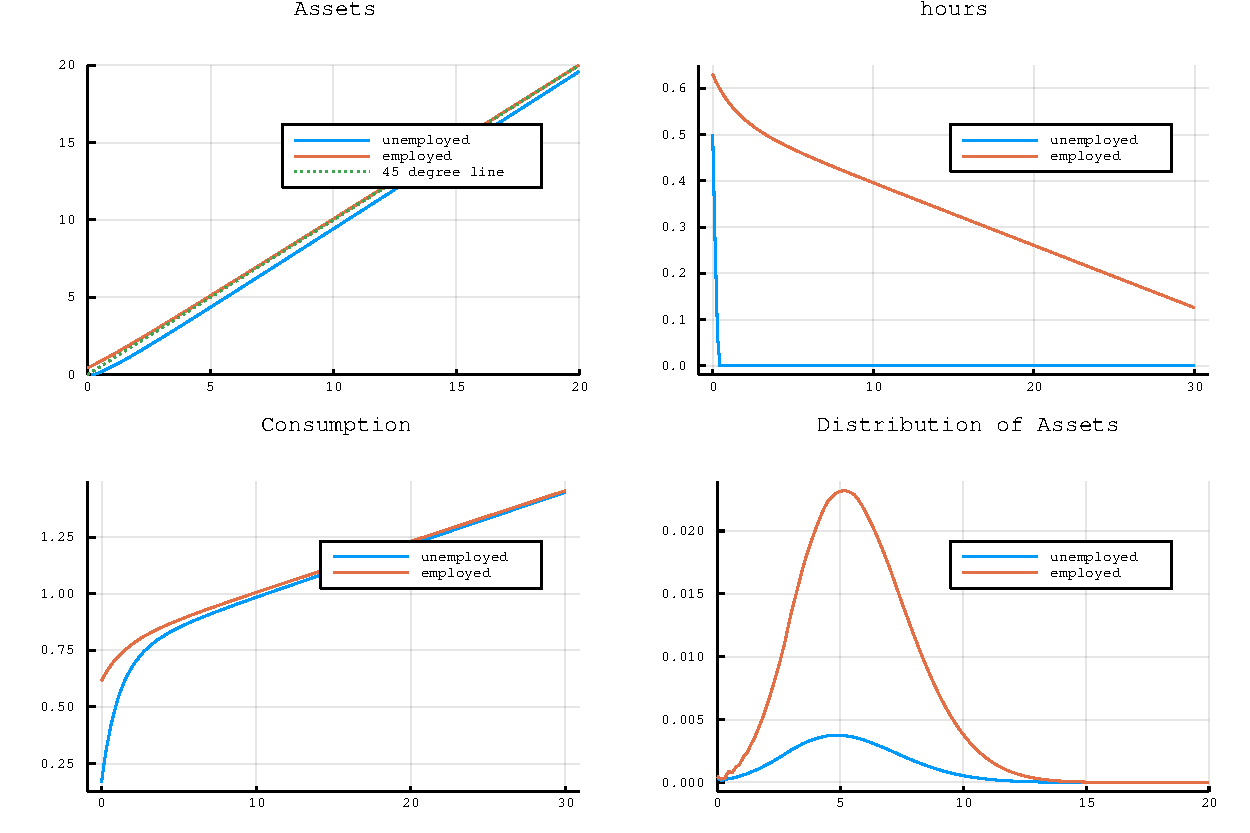
\includegraphics[width = 0.8\textwidth]{../ElasticLabor/Solution2.pdf}
    \caption{$\gamma_c = \gamma_l = 1.0$ and $\beta = 0.96$}
  \end{figure}
%%%%
  Introducing valued leisure to the model created several computational challenges. First of all, while solving the individual problem, we had to also solve for labor through the marginal rate of intratemporal substitution (both in the current period and in every state of next period). Further, instead of merely solving for a market clearing interest rate, we also had to solve for a market clearing wage rate. Conveniently, this market clearing wage rate can be solved in a newton whose update happens after clearing capital markets. With a newton, we get quadratic convergence, so clearing both market does not increase computational burdens that much.
  Figure 2 displays solutions to the benchmark case with valued leisure. We can see that with valued leisure, under the low income shock, even though labor income is worth very little, the agent will still work under very low asset levels in order to be able to consume. You can also see the difference in the policy function which now doesn't look as parallel as the one in the exogenous labor case. The idea here is that at higher asset levels, high labor income agent can also work less as means of increasing his/her utility so won't need to save as much compared to the low labor income agent. Finally, the aggregate capital was 5.62 and aggregate labor was 0.396. \\
  \\
  %%%%%%%%%%%%%%%%%%%%%%%
\begin{figure}[h!]
  \centering
  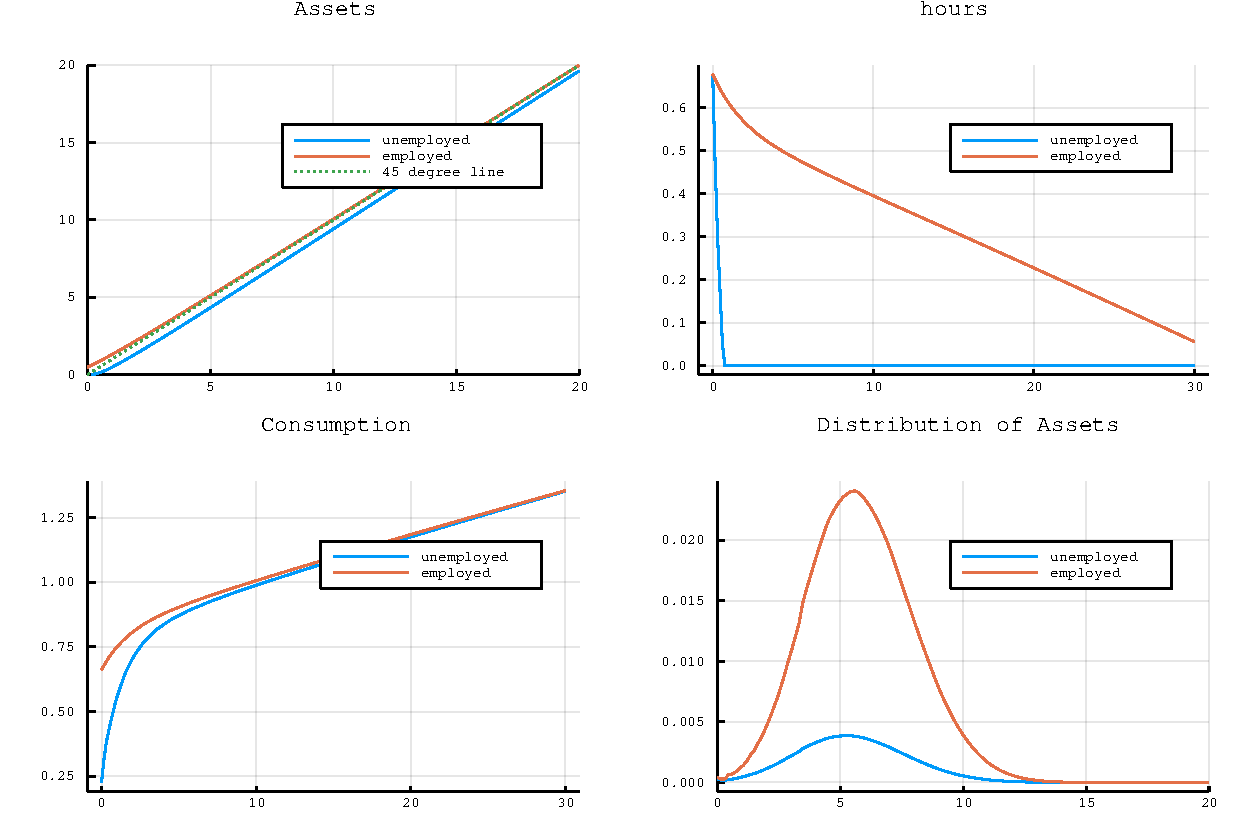
\includegraphics[width = 0.8\textwidth]{../ElasticLabor/Solution.pdf}
    \caption{$\gamma_c = 1.5$, $\gamma_l = 1.0$ and $\beta = 0.96$}
  \end{figure}
  Figure 3 displays the second case with valued leisure where we increased the elasticity of consumption to 1.5 to see how results differ. The pattern is the same as that in Marcet et al (2006). In other words, we get a higher aggregate capital and labor (5.79 and 0.405 respectively) as we increase the elasticity of consumption and agents want to save more to buffer risk (loosing consumption becomes more costly). This can also be seen in the policy function for labor where now that the agent is more risk averse, at low labor income values, the agent will work more relative to the low $\gamma_c$ case.  \\
  \\
  %%%%%%%%%%%%%%%%%%%%%%%
\begin{figure}[h!]
  \centering
  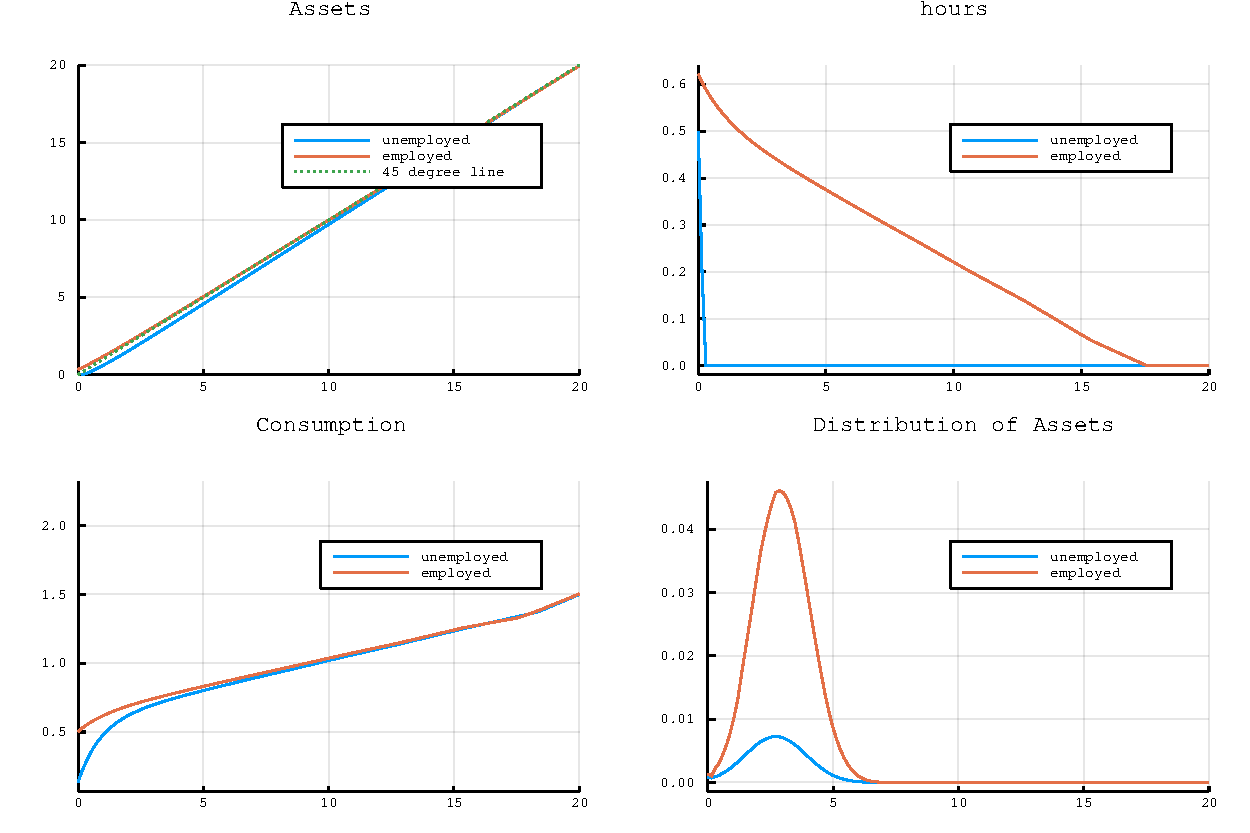
\includegraphics[width = 0.8\textwidth]{../ElasticLabor/Solution3.pdf}
    \caption{$\gamma_c = 1.0$, $\gamma_l = 1.0$ and $\beta = 0.93$}
  \end{figure}
  Figure 4 displays results from our last case where I slashed the discount factor to illustrate an economy with very low discount factors. As one would predict, agents start disaving quite fast as they discount the future more and the aggregate level of capital is significantly low. All in all,   
  

















\end{document}
